%!TEX root = ../thesis.tex
%*******************************************************************************
%*********************************** First Chapter *****************************
%*******************************************************************************

\chapter{Introduction}  %Title of the First Chapter

\ifpdf
    \graphicspath{{Chapter1/Figs/Raster/}{Chapter1/Figs/PDF/}{Chapter1/Figs/}}
\else
    \graphicspath{{Chapter1/Figs/Vector/}{Chapter1/Figs/}}
\fi


\section{What is helioseismology?} %Section - 1.1 
Helioseismology is the study of structure and internal dynamics of the sun as a system by analysing its oscillations. It was discovered in 1960 that a time series of solar dopplegram images reveal global oscillasions in line of sight velocity with well defined frequencies \cite{Kosovichev2011}. Most of observational helioseismic data is that of oscillations of the of solar material manifesting on the surface \cite{jcd_notes}. A Dopplergram image is an image of sun formed by measuring doppler shift of a predetermined atomic spectral line and assigning a line-of-sight velocity to the corresponding pixel. After arranging all the pixels one obtains a map of the line of sight velocity of the sun in an instant of time like figure (\ref{fig:sun_doppler}). A number of dopplergram images can be arranged in time order to form a `time series'. This time series allows us to process this data to obtain either frequency spectra (for global helioseismology), or time-distance measurements (for local helioseismology).

Global helioseismology attempts to probe the internal structure of the sun by analysing stochastically excited resonant acoustic  modes and their corresponding frequencies. While local helioseismology attempts to achive this goal via analysis of wavefield cross-correlations and travel times on the solar surface \cite{gizon02}.
\begin{figure}[h]
\includegraphics[scale=0.5,center]{Chapter1/figs/sun_doppler}
\caption{Typical dopplergram image of sun showing line of sight velocity as the color field. Rotational profile of sun is clearly visible. Image taken by Michelson Doppler Imager aboard SOHO spacecraft. Image obtained from \cite{Kosovichev2011}.}
\label{fig:sun_doppler}
\end{figure}

\section{Overview}
In the second chapter, we motivate and develop the prerequisite techniques which are widely used in the rest of the work. We describe the standard model of the sun that we consider as a background model in this work. Next we describe briefly the method of quasi-degenerate perturbation theory that we use repeatedly to find frequency corrections of closely placed modes as a result of mode-coupling. We also discuss the standard way of representing splitting data in helioseismology.

In the third and fourth chapters, we discuss coupling of modes due to differential rotation and magnetic fields respectively. The last chapter is devoted to quoting and discussing the results of our analysis.
\chapter{Formalism}

\section{Standard Model and Frequency splittings} %Section - 1.2p
\subsection{Background equation of motion}
The standard solar model assumed in this work is that of a spherically symmetric, non-rotating, non-magnetic, adiabatic, isotropic, and static (\snr). When equations of motion solved for displacement field $\xiv$ about the static equilibrium configuration, the \snr model is found to admit wavelike solutions in displacement obeying the following differential equation in temporal frequency domain.

\begin{equation} \label{eqn:sol_wave_eqn}
\cL_0 \xiv  \equiv - \grad (\rho c^2 \boldsymbol{\nabla} \cdot \boldsymbol{\xi} - \rho g \boldsymbol{\xi} \cdot \ev{r}) - g \ev{r} \boldsymbol{\nabla} \cdot (\rho \boldsymbol{\xi}) = \rho \omega^2 \xiv
\end{equation}


where $\omega$ denotes the temporal frequency of the oscillation, $c(r)$ is the sound speed profile, $-g(r)\ev{r}$ is the graviational field, $\rho(r)$ is mass density and $\ev{r}$ is the radial unit vector. For all ensuing calculations and derivations we write equation (\ref{eqn:sol_wave_eqn}) in the form $\mathcal{L}_0 \boldsymbol{\xi} = \rho \omega^2 \boldsymbol{\xi}$ which is to be understood as an eigenvalue equation with the eigenvalue $\omega^2$. It can be shown that the unperturbed wave operator $\mathcal{L}_0$ is self-adjoint \cite{goedbloed2004}. Flow fields, rotations, asphericities, anisotropies and non-radial variations in $c, g, \rho$ can be captured as perturbation terms in equation (\ref{eqn:sol_wave_eqn}). Although for the purpose of this study, we shall restrict ourselves to perturbations induced via presence of an axisymmetric flow (differential rotation) global scale magnetic fields only.

Since the operator $\cL_0$ is self-adjoint, it has a complete set of eigenfunctions and corrrespoding quantised set of eigenfrequencies. These eigenfunctions and corresponding eigenfrequencies are called \textit{normal modes} and \textit{resonant frequencies} respectively. After decomposing the displacement field $\xiv$ into vector spherical harmonics it can be shown that eigenfunctions are characterised by three quantum numbers known as the radial order $n$, harmonic degree $l$ and azimuthal order $m$. The eigenvalue equation in then given by

\begin{equation}
\cL_{0}\xiv_{nlm} = \rho \omega_{nl}^2 \xiv_{nlm}
\end{equation}

where $\omega_{nl}$ is the eigenfrequency of the mode $\xiv_{nlm}$. As consequence of the spherical symmetry, the eigenfrequencies $\omega_{nlm}$ are independent of the azimuthal quantum number $m$ and are thus given by $\omega_{nl}$. When any internal structure parameter such as convective flow, differential rotation, magnetic fields etc is introduced in the description of the system, they can be treated as a departure from the \snr model. This leads to a lifting in the degeneracy in mode frequencies $\omega_{nl}$. These frequency splitting can be calculated via a pertubative analysis of the $\cL_0$ operator and its spectrum. The \textit{forward problem} in global helioseismology is to find the relation between these split frequencies and these internal parameters. The essential idea of the \textit{inverse problem} is to systematically deduce these internal structure parameters from frequency splittings of solar acoustic resonant modes.

\subsection{Form of eigenfunction}
A vector spherical harmonic decomposition of a vector field $\mathbf{A}(\rvec)$ is given as 
\begin{equation}
\mathbf{A}(\rvec) = \sum_{lm} \encsqr{U_{lm}(r) Y_l^m \ev{r} + V_{lm}(r) \grad_{1}Y_l^m + W_{lm}(r) \ev{r} \times \grad_1 Y_{l}^{m}}
\end{equation}
where $\boldsymbol{r} = (r,\theta,\phi)$ in spherical polar coordinate system with basis vectors $(\ev{r},\ev{\theta},\ev{\phi})$, $\grad_1 \equiv = \enc{\ev{\theta}\partial_{\theta} + \ev{\phi}\frac{1}{\sin\theta}\partial_{\phi} }$. Here, the first two parts involving $U_{ml}$ and $V_{lm}$ constitute the \textit{spheroidal} (or poloidal) component and the last part is constitutes the \textit{toroidal} component. Note that the spheroidal component has zero curl (irrotational) and the toroidal part has zero divergence (solenoidal).

Since the sun is essentially a fluid system, it is capable of offering restoring stress in response (and in proportion) to \textit{shear strain rate} (shearing viscosity) but no restoring stress in response to \textit{shear strain}, unlike the earth. This leads to the solar eigenfunctions lacking a toroidal component ($\ev{r}\times \grad_1 Y_{l}^m$) \cite{jcd_notes}. Hence, they have the form
\begin{eqnarray} \label{eqn: xi_exp}
    \boldsymbol{\xi}_{nlm}(\boldsymbol{r}) =  U_{nl}(r) Y_l^m(\theta,\phi) \ev{r}
 + V_{nl}(r) \boldsymbol{\nabla}_1 Y_l^m(\theta,\phi)
\end{eqnarray}
 
The entire set of $(2l+1)$ degenerate \snr eigenmodes having unperturbed frequency $\omega_{nl}$ is called $\mode{n}{l}$ where the $S$ stands for `spheroidal'. This nomenclature borrows from the `spheroidal + toroidal' decomposition of vector fields where the former is irrotational and the latter is solenoidal \cite{lavely92}. In geophysics literature, one also encounters toroidal modes $_nT_l$ \cite{DT98}.

We work with normalised eigenfunctions $\boldsymbol{\xi}_k$ with the spherically symmetric background density $\rho(r)$ as the weight factor, which satisfy the orthonormality condition:

\begin{equation} \label{eqn: orthonormality}
  \inner{\xiv_{k'}}{\rho\xiv_{k}} = \delta_{n'n} \delta_{l' l} \delta_{m' m}  
\end{equation}
where $k = (n,l,m)$, and the inner product \inner{}{} stands for $\inner{\Phi}{\Psi} \equiv \ints d^3\rvec \Phi^*(\rvec)\cdot \Psi(\rvec)$.

\section{Quasi Degenerate Perturbation Theory}
Quasi-degenerate perturbation theory (QDPT) requires us to account for mixing of modes which lie in a small neighbourhood on the frequency spectrum, and hence satisfy the quasi-degenerate condition
\begin{equation}\label{eqn:qdpt_cond}
|\omega_k^2 - \omref^2| < \tau^2
\end{equation}
where $\omega_{ref}$ is some reference frequency defining the centre of the frequency interval. At the end of the section we'll demonstrate that degenerate perturbation theory (DPT) is a special case of QDPT.

Consider a set of multiplets $\mode{n}{l}$ lying close enough on the frequency spectrum to satisfy the quasi-degenerate condition (\ref{eqn:qdpt_cond}). Let the entire space spanned by these functions be called $\cK$. Then, as a perturbation $\cL \rightarrow \cL + \delta\cL$ is introduced, the following changes are also introduced into the system
\begin{equation}
\xiv_k \rightarrow \tilde{\xiv} + \delta\txiv
\end{equation}
\begin{equation}
\omega_{k}^2 \rightarrow \omega_{ref}^2 + \domsq
\end{equation}

where $\tilde{\xiv}$ is a linear combination of all the modes in $\cK$ given by $\xiv = \sum_{k \in \cK} c_k \xiv_{k}$ and $\delta \txiv$ is a correction vector lying in $\cK'$ which is the orthogonal space of $\cK$. Now, the new perturbed equation of motion is written as

\begin{equation}
\enc{\cL + \delta \cL} \enc{\txiv + \delta\txiv} = \rho \enc{\omref^2 + \domsq} \enc{\txiv + \delta\txiv}
\end{equation}

Expanding above equation and taking an inner product on both sides with $\xiv_k$ gives
\begin{equation}\label{eqn:qdpt_eig}
\sum_{k'\in \cK} Z_{kk'} c_{k'} = \domsq c_{k}
\end{equation}
where $Z_{k'k}$ is the supermatrix defined as 
\begin{equation}
Z_{k'k} \equiv \inner{\xiv_{k'}}{\dL\xiv_{k}} - \delta_{k'k} (\omref^2 - \omega_{k}^2)
\end{equation}
We can see that the leading order correction in eigenfrequency is given by the eigenvalues to the supermatrix $Z_{k'k}$ in equation (\ref{eqn:qdpt_eig}). We also find that $\txiv$ can be recovered as its decomposition coefficients in $\cK$ space is described by the eigenvectors of the supermatrix.

Note: The quantity $\inner{\xiv_{k'}}{\dL\xiv{k}}$ will be referred to as the coupling matrix $\Lambda_{k'k}$ throughout this work to reduce notational burden.

Finally, as a corollary of the theory developed above, let us consider the case of $\cK$ consisting of modes that are all degenerate with frequency $\omega_0$. In this case, setting $\omref = \omega_0$, we see that $Z_{k'k}$ reduces to $\Lambda_{k'k}$. Now the leading order corrections to eigenfrequency and eigenfunction are described by eigenvalue and eigenvectors of $\Lambda_{k'k}$; this is known as degenerate perturbation theory (DPT). A more detailed version of this analysis can be found in \cite{lavely92}.


\section{Representation of Splitting Data}
Since each multiplet $\mode{n}{l}$ contains $2l+1$ singlet modes, it is tedious to give the degree of splitting in the mode by exact value of each split frequency $\omega_{nlm}$ by itself. Therefore, in helioseismology, splitting data is represented by numbers called splitting coefficients which describe the decomposition of $\delta\omega_{nlm} = \omega_{nlm}-\omega_{nl}$ in terms of some basis function over $m$ as follows
\begin{equation}
\omega_{nlm} = \omega_{nl} + \sum_{j=0}^{j_{max}} a^{nl}_j \cP_j(m)
\label{eq:a_def}
\end{equation}
where $\cP_{j}(m)$ with $j\in \{0,1,2,\ldots, j_{max}\}$ represents a $j_{max}+1$ dimensional orthogonal basis function of polynomials on the discrete space of $m$'s which run from $-l$ to $l$. Since, there are $2l+1$ points in this discrete domain, the (vector) space spanned by all functions on this domain is $(2l+1)$ dimensional, which in turn means $j_{max}$ cannot exceed $2l$. In practice, $a$-coefficients are recorded till a $j_{max}$ of $10$ (\cite{schou_data} for instace). We will use, as a standard, the basis functions prescribed in \cite{ritzwoller} which are Gram-Schmidt orthogonalised polynomials of increasing degree starting with $\cP_0(m) = l$. Given the normalisation condition mentioned above, and this starting condition, the polynomials become well defined. A recipe for obtaining these can be found in Appendix A of \cite{schou_pol_94}. Some properties to note about these polynomials are
\begin{itemize}
\item $\cP_j(m)$ is odd/even about $m=0$ if $j$ is odd/even respectively.
\item $\cP_j(m)$ has polynomial degree $j$ in $m$.
\item $\cP_j(m)$ contains only odd/even powers of $m$ if $j$ is odd/even respectively.
\item In limit $l \gg 1$, $\cP_j(m) \approx lP_{j}(m/l)$, where $P_j$ is Legendre polynomial of degree $j$.
\end{itemize}

Once we have the splitting data $\omega_{nlm}$, one can easily compute the $a$ coefficients multiplying both sides of Eq.(\ref{eq:a_def}) by $\cP_k(m)$,summing over all $m$, and finally using using the orthogonality condition $$\sum_{m=-l}^l \cP_{j}(m) \cP_{k}(m) = \delta_{jk} \sum_{m=-l}^l \enc{\cP_{j}(m)}^2$$
as

\begin{equation}
a^{nl}_j = \sum_{m=-l}^l \delta\omega_{nlm}\cP_j(m) \bigg/ \sum_{m=-l}^l \enc{\cP_j(m)}^2
\end{equation}


Note that, even though scaled Legendre polynomials $lP_j(m/l)$ are not perfectly orthogonal on a discretised domain (under the inner product $(A|B)\sum_{m=-l}^l A^*(m)B(m)$), they are still linearly independent. However their use should be avoided as a basis to represent splitting data because value of $a$-coefficients will change slightly depending on $j_{max}$, i.e. how many $a$ coefficients are being fitted to the data; this occurs due to non-zero inner product between different basis functions. An orthogonal basis like $\cP_j$ solves this issue by making $a_j$ values independent of $j_{max}$.

Thus, henceforth whenever `$a$-coefficients' are referred to in this text, it shall be understood that the underlying basis functions are given by $\{\cP_j: j\in \{0,1,\dots,j_{max}\}\}$. The first three $\cP$s are given below.

\begin{align}
\cP_{0}(m) &= l \\
\cP_1(m) &= m \\
\cP_2(m) &= \frac{3m^2-l(l+1)}{2l-1}
\end{align}

Figure (\ref{fig:curly_p}) shows that $\cP_j(m)$ bear close resemblance with scaled Legendre polynomials $lP(m/l)$.
\begin{figure}[h]
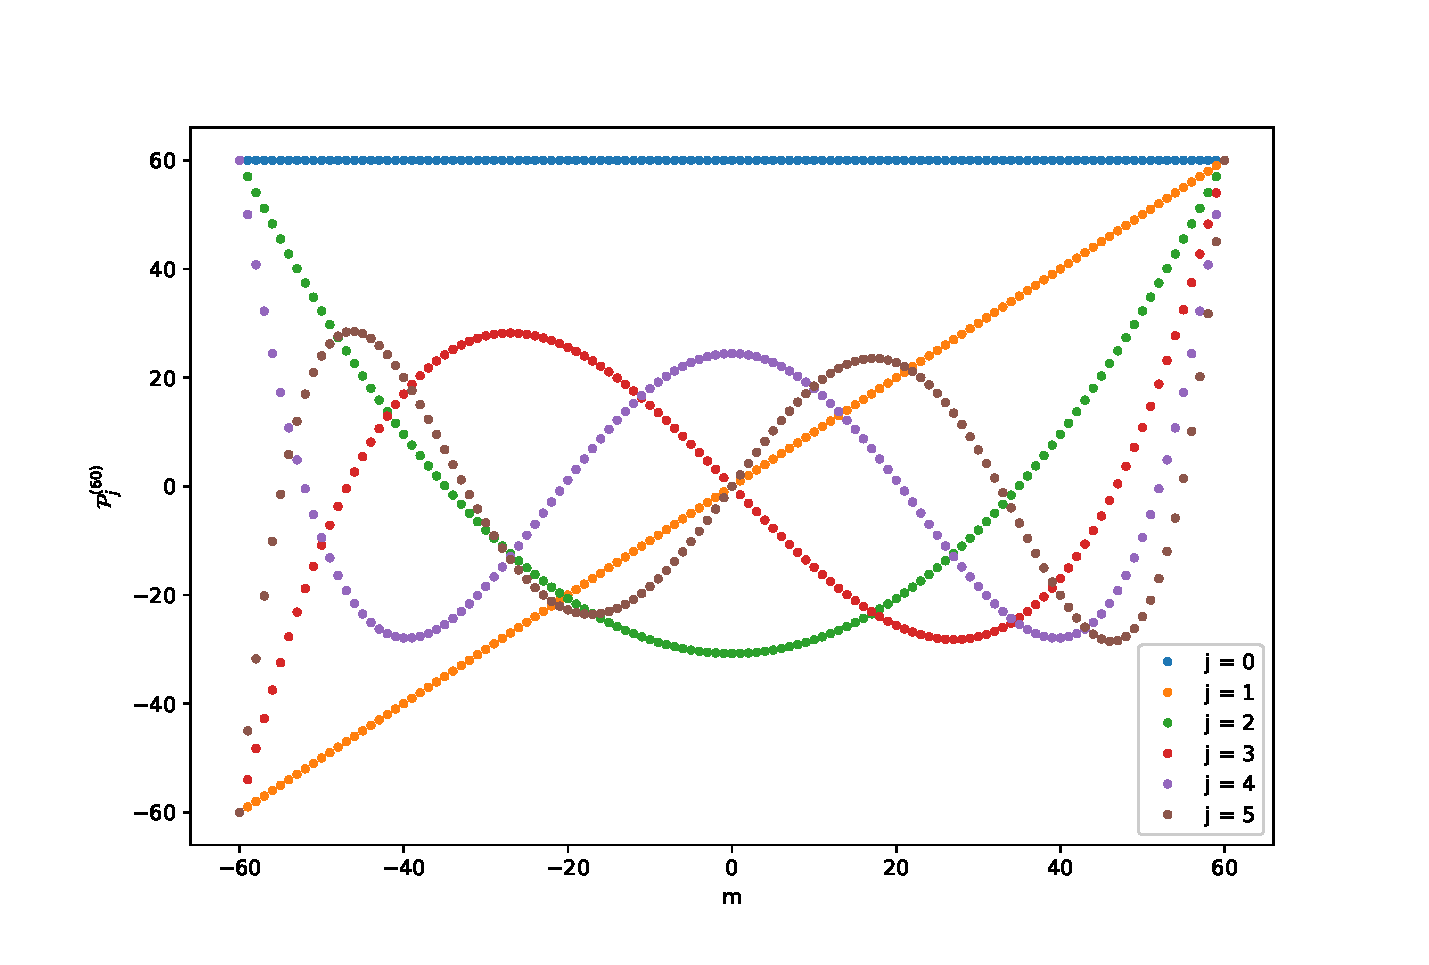
\includegraphics[scale=0.6, center]{Chapter1/figs/curly_p}
\caption{Orthogonal basis functions $\cP_{j}$ upto $j=5$ for $l=60$.}\
\label{fig:curly_p}
\end{figure}
